\documentclass[twoside]{book}

% Packages required by doxygen
\usepackage{fixltx2e}
\usepackage{calc}
\usepackage{doxygen}
\usepackage[export]{adjustbox} % also loads graphicx
\usepackage{graphicx}
\usepackage[utf8]{inputenc}
\usepackage{makeidx}
\usepackage{multicol}
\usepackage{multirow}
\PassOptionsToPackage{warn}{textcomp}
\usepackage{textcomp}
\usepackage[nointegrals]{wasysym}
\usepackage[table]{xcolor}

% Font selection
\usepackage[T1]{fontenc}
\usepackage[scaled=.90]{helvet}
\usepackage{courier}
\usepackage{amssymb}
\usepackage{sectsty}
\renewcommand{\familydefault}{\sfdefault}
\allsectionsfont{%
  \fontseries{bc}\selectfont%
  \color{darkgray}%
}
\renewcommand{\DoxyLabelFont}{%
  \fontseries{bc}\selectfont%
  \color{darkgray}%
}
\newcommand{\+}{\discretionary{\mbox{\scriptsize$\hookleftarrow$}}{}{}}

% Page & text layout
\usepackage{geometry}
\geometry{%
  a4paper,%
  top=2.5cm,%
  bottom=2.5cm,%
  left=2.5cm,%
  right=2.5cm%
}
\tolerance=750
\hfuzz=15pt
\hbadness=750
\setlength{\emergencystretch}{15pt}
\setlength{\parindent}{0cm}
\setlength{\parskip}{3ex plus 2ex minus 2ex}
\makeatletter
\renewcommand{\paragraph}{%
  \@startsection{paragraph}{4}{0ex}{-1.0ex}{1.0ex}{%
    \normalfont\normalsize\bfseries\SS@parafont%
  }%
}
\renewcommand{\subparagraph}{%
  \@startsection{subparagraph}{5}{0ex}{-1.0ex}{1.0ex}{%
    \normalfont\normalsize\bfseries\SS@subparafont%
  }%
}
\makeatother

% Headers & footers
\usepackage{fancyhdr}
\pagestyle{fancyplain}
\fancyhead[LE]{\fancyplain{}{\bfseries\thepage}}
\fancyhead[CE]{\fancyplain{}{}}
\fancyhead[RE]{\fancyplain{}{\bfseries\leftmark}}
\fancyhead[LO]{\fancyplain{}{\bfseries\rightmark}}
\fancyhead[CO]{\fancyplain{}{}}
\fancyhead[RO]{\fancyplain{}{\bfseries\thepage}}
\fancyfoot[LE]{\fancyplain{}{}}
\fancyfoot[CE]{\fancyplain{}{}}
\fancyfoot[RE]{\fancyplain{}{\bfseries\scriptsize Generated by Doxygen }}
\fancyfoot[LO]{\fancyplain{}{\bfseries\scriptsize Generated by Doxygen }}
\fancyfoot[CO]{\fancyplain{}{}}
\fancyfoot[RO]{\fancyplain{}{}}
\renewcommand{\footrulewidth}{0.4pt}
\renewcommand{\chaptermark}[1]{%
  \markboth{#1}{}%
}
\renewcommand{\sectionmark}[1]{%
  \markright{\thesection\ #1}%
}

% Indices & bibliography
\usepackage{natbib}
\usepackage[titles]{tocloft}
\setcounter{tocdepth}{3}
\setcounter{secnumdepth}{5}
\makeindex

% Hyperlinks (required, but should be loaded last)
\usepackage{ifpdf}
\ifpdf
  \usepackage[pdftex,pagebackref=true]{hyperref}
\else
  \usepackage[ps2pdf,pagebackref=true]{hyperref}
\fi
\hypersetup{%
  colorlinks=true,%
  linkcolor=blue,%
  citecolor=blue,%
  unicode%
}

% Custom commands
\newcommand{\clearemptydoublepage}{%
  \newpage{\pagestyle{empty}\cleardoublepage}%
}

\usepackage{caption}
\captionsetup{labelsep=space,justification=centering,font={bf},singlelinecheck=off,skip=4pt,position=top}

%===== C O N T E N T S =====

\begin{document}

% Titlepage & ToC
\hypersetup{pageanchor=false,
             bookmarksnumbered=true,
             pdfencoding=unicode
            }
\pagenumbering{alph}
\begin{titlepage}
\vspace*{7cm}
\begin{center}%
{\Large Rookie Tales \\[1ex]\large 2.\+0 }\\
\vspace*{1cm}
{\large Generated by Doxygen 1.8.13}\\
\end{center}
\end{titlepage}
\clearemptydoublepage
\pagenumbering{roman}
\tableofcontents
\clearemptydoublepage
\pagenumbering{arabic}
\hypersetup{pageanchor=true}

%--- Begin generated contents ---
\chapter{Class Index}
\section{Class List}
Here are the classes, structs, unions and interfaces with brief descriptions\+:\begin{DoxyCompactList}
\item\contentsline{section}{\hyperlink{structBackground}{Background} }{\pageref{structBackground}}{}
\item\contentsline{section}{\hyperlink{structButton}{Button} }{\pageref{structButton}}{}
\item\contentsline{section}{\hyperlink{structDialogue}{Dialogue} }{\pageref{structDialogue}}{}
\item\contentsline{section}{\hyperlink{structenigme}{enigme} }{\pageref{structenigme}}{}
\item\contentsline{section}{\hyperlink{structEnigme}{Enigme} \\*Structure pour l\textquotesingle{}enigme math(numero 1) }{\pageref{structEnigme}}{}
\item\contentsline{section}{\hyperlink{structEntite}{Entite} }{\pageref{structEntite}}{}
\item\contentsline{section}{\hyperlink{structHeart}{Heart} }{\pageref{structHeart}}{}
\item\contentsline{section}{\hyperlink{structHero}{Hero} \\*Structure de l\textquotesingle{}hero qui utilise d\textquotesingle{}autres structures définies (sprite, vie et score) et des enum (direction et state) }{\pageref{structHero}}{}
\item\contentsline{section}{\hyperlink{structHeure}{Heure} }{\pageref{structHeure}}{}
\item\contentsline{section}{\hyperlink{structMatchstick}{Matchstick} }{\pageref{structMatchstick}}{}
\item\contentsline{section}{\hyperlink{structMinimap}{Minimap} }{\pageref{structMinimap}}{}
\item\contentsline{section}{\hyperlink{structParameter}{Parameter} }{\pageref{structParameter}}{}
\item\contentsline{section}{\hyperlink{structPlatforme}{Platforme} }{\pageref{structPlatforme}}{}
\item\contentsline{section}{\hyperlink{structPortal}{Portal} }{\pageref{structPortal}}{}
\item\contentsline{section}{\hyperlink{structPower__up}{Power\+\_\+up} }{\pageref{structPower__up}}{}
\item\contentsline{section}{\hyperlink{structScore}{Score} }{\pageref{structScore}}{}
\item\contentsline{section}{\hyperlink{structSprite}{Sprite} \\*Ustilisé dans la fonction animer\+\_\+hero en parcourant le spritesheet selon S\+T\+A\+TE de l\textquotesingle{}hero }{\pageref{structSprite}}{}
\item\contentsline{section}{\hyperlink{structSprite__entite}{Sprite\+\_\+entite} }{\pageref{structSprite__entite}}{}
\item\contentsline{section}{\hyperlink{structText}{Text} }{\pageref{structText}}{}
\item\contentsline{section}{\hyperlink{structText__enigme}{Text\+\_\+enigme} }{\pageref{structText__enigme}}{}
\item\contentsline{section}{\hyperlink{structTimer}{Timer} }{\pageref{structTimer}}{}
\item\contentsline{section}{\hyperlink{structVie}{Vie} }{\pageref{structVie}}{}
\end{DoxyCompactList}

\chapter{Class Documentation}
\hypertarget{structBackground}{}\doxysection{Background Struct Reference}
\label{structBackground}\index{Background@{Background}}
\doxysubsection*{Data Fields}
\begin{DoxyCompactItemize}
\item 
\mbox{\Hypertarget{structBackground_a637e6c83f05e045ce23bda645cdd8574}\label{structBackground_a637e6c83f05e045ce23bda645cdd8574}} 
S\+D\+L\+\_\+\+Surface $\ast$ {\bfseries image}
\item 
\mbox{\Hypertarget{structBackground_a3d66779716725a2f8377aaed0eb374b2}\label{structBackground_a3d66779716725a2f8377aaed0eb374b2}} 
S\+D\+L\+\_\+\+Surface $\ast$ {\bfseries foreground}
\item 
\mbox{\Hypertarget{structBackground_ac76c2da4307e469688a1286d4ac70842}\label{structBackground_ac76c2da4307e469688a1286d4ac70842}} 
S\+D\+L\+\_\+\+Surface $\ast$ {\bfseries background\+\_\+mask}
\item 
\mbox{\Hypertarget{structBackground_a6a43437543c71a78285c8049b5cb3dc0}\label{structBackground_a6a43437543c71a78285c8049b5cb3dc0}} 
S\+D\+L\+\_\+\+Rect {\bfseries position\+\_\+background\+\_\+mask}
\item 
\mbox{\Hypertarget{structBackground_a41d570eb769454b0488aeccd9e4970a2}\label{structBackground_a41d570eb769454b0488aeccd9e4970a2}} 
S\+D\+L\+\_\+\+Rect {\bfseries pos\+Camera}
\item 
\mbox{\Hypertarget{structBackground_afa1e935c412a4c4154f5c3e2b7b93791}\label{structBackground_afa1e935c412a4c4154f5c3e2b7b93791}} 
S\+D\+L\+\_\+\+Rect {\bfseries pos\+\_\+foreground}
\item 
\mbox{\Hypertarget{structBackground_a57b869b301c9c1e8f69c9abee7e00b2a}\label{structBackground_a57b869b301c9c1e8f69c9abee7e00b2a}} 
S\+D\+L\+\_\+\+Surface $\ast$ {\bfseries platform}
\item 
\mbox{\Hypertarget{structBackground_af35046bf47fc0b707d62020227b58720}\label{structBackground_af35046bf47fc0b707d62020227b58720}} 
S\+D\+L\+\_\+\+Rect {\bfseries pos\+\_\+platform}
\end{DoxyCompactItemize}


The documentation for this struct was generated from the following file\+:\begin{DoxyCompactItemize}
\item 
background.\+h\end{DoxyCompactItemize}

\hypertarget{structButton}{}\doxysection{Button Struct Reference}
\label{structButton}\index{Button@{Button}}
\doxysubsection*{Data Fields}
\begin{DoxyCompactItemize}
\item 
\mbox{\Hypertarget{structButton_a9b46ba5cac45b47ada9d1491ffff575d}\label{structButton_a9b46ba5cac45b47ada9d1491ffff575d}} 
S\+D\+L\+\_\+\+Surface $\ast$ {\bfseries image}
\item 
\mbox{\Hypertarget{structButton_a0343ba330902623017b8915e2d629a83}\label{structButton_a0343ba330902623017b8915e2d629a83}} 
S\+D\+L\+\_\+\+Rect {\bfseries position}
\end{DoxyCompactItemize}


The documentation for this struct was generated from the following file\+:\begin{DoxyCompactItemize}
\item 
menu.\+h\end{DoxyCompactItemize}

\hypertarget{structDialogue}{}\section{Dialogue Struct Reference}
\label{structDialogue}\index{Dialogue@{Dialogue}}


Collaboration diagram for Dialogue\+:

\hypertarget{structenigme}{}\section{enigme Struct Reference}
\label{structenigme}\index{enigme@{enigme}}
\subsection*{Public Attributes}
\begin{DoxyCompactItemize}
\item 
\mbox{\Hypertarget{structenigme_afef580eaca259227dac7bbae2d09f8f7}\label{structenigme_afef580eaca259227dac7bbae2d09f8f7}} 
S\+D\+L\+\_\+\+Surface $\ast$ {\bfseries background}
\item 
\mbox{\Hypertarget{structenigme_a10ee397636fe45d16379476fb990c58a}\label{structenigme_a10ee397636fe45d16379476fb990c58a}} 
S\+D\+L\+\_\+\+Surface $\ast$ {\bfseries bgansewr}
\item 
\mbox{\Hypertarget{structenigme_aebbf2d7046b5e0545f7b84fef6e98831}\label{structenigme_aebbf2d7046b5e0545f7b84fef6e98831}} 
S\+D\+L\+\_\+\+Surface $\ast$ {\bfseries bghover}
\item 
\mbox{\Hypertarget{structenigme_a917462fa7abd51385bfb39274d24c11f}\label{structenigme_a917462fa7abd51385bfb39274d24c11f}} 
S\+D\+L\+\_\+\+Surface $\ast$ {\bfseries Question}
\item 
\mbox{\Hypertarget{structenigme_ab3a0b156348a72483447216e90c28af0}\label{structenigme_ab3a0b156348a72483447216e90c28af0}} 
S\+D\+L\+\_\+\+Surface $\ast$ {\bfseries ansewr1}
\item 
\mbox{\Hypertarget{structenigme_a97c066a4114758708b5b4400f07de023}\label{structenigme_a97c066a4114758708b5b4400f07de023}} 
S\+D\+L\+\_\+\+Surface $\ast$ {\bfseries ansewr2}
\item 
\mbox{\Hypertarget{structenigme_a49754c0a7b2de36218e07574b0df6ea4}\label{structenigme_a49754c0a7b2de36218e07574b0df6ea4}} 
S\+D\+L\+\_\+\+Surface $\ast$ {\bfseries ansewr3}
\item 
\mbox{\Hypertarget{structenigme_a4eb7509adf07f09049e9a375d249bea6}\label{structenigme_a4eb7509adf07f09049e9a375d249bea6}} 
S\+D\+L\+\_\+\+Surface $\ast$ {\bfseries ansewr4}
\item 
\mbox{\Hypertarget{structenigme_ad4909b90c50cc4caf5d702e18f83e335}\label{structenigme_ad4909b90c50cc4caf5d702e18f83e335}} 
S\+D\+L\+\_\+\+Surface $\ast$ {\bfseries Yes}
\item 
\mbox{\Hypertarget{structenigme_a630ac6f3949179ec340c9e71ad53faee}\label{structenigme_a630ac6f3949179ec340c9e71ad53faee}} 
S\+D\+L\+\_\+\+Surface $\ast$ {\bfseries No}
\item 
\mbox{\Hypertarget{structenigme_a38e749d7ae027b8a4b487a49b49fe671}\label{structenigme_a38e749d7ae027b8a4b487a49b49fe671}} 
S\+D\+L\+\_\+\+Surface $\ast$ {\bfseries Final}
\item 
\mbox{\Hypertarget{structenigme_ae0dd357e0952647ab0de64abc803b660}\label{structenigme_ae0dd357e0952647ab0de64abc803b660}} 
S\+D\+L\+\_\+\+Rect {\bfseries position\+Background}
\item 
\mbox{\Hypertarget{structenigme_abd09b99260062e8b2f5ec41c9eedbfae}\label{structenigme_abd09b99260062e8b2f5ec41c9eedbfae}} 
S\+D\+L\+\_\+\+Rect {\bfseries position\+Ansewr1}
\item 
\mbox{\Hypertarget{structenigme_a64fefb6cab2baaee1c0e54d51f4b5486}\label{structenigme_a64fefb6cab2baaee1c0e54d51f4b5486}} 
S\+D\+L\+\_\+\+Rect {\bfseries position\+Ansewr2}
\item 
\mbox{\Hypertarget{structenigme_aba195f6df5f2e975e2bb19983f2ae542}\label{structenigme_aba195f6df5f2e975e2bb19983f2ae542}} 
S\+D\+L\+\_\+\+Rect {\bfseries position\+Ansewr3}
\item 
\mbox{\Hypertarget{structenigme_a5b5c3043e61541f4c63c1bc55651ca51}\label{structenigme_a5b5c3043e61541f4c63c1bc55651ca51}} 
S\+D\+L\+\_\+\+Rect {\bfseries position\+Ansewr4}
\item 
\mbox{\Hypertarget{structenigme_ae10e2d3b647b0728eba96dcbc3098619}\label{structenigme_ae10e2d3b647b0728eba96dcbc3098619}} 
S\+D\+L\+\_\+\+Rect {\bfseries positionQ}
\item 
\mbox{\Hypertarget{structenigme_acbf34a299f6a43366abb738df85c282d}\label{structenigme_acbf34a299f6a43366abb738df85c282d}} 
S\+D\+L\+\_\+\+Rect {\bfseries positionhover}
\item 
\mbox{\Hypertarget{structenigme_a53787af725dae2956717fa2eba7ca6a9}\label{structenigme_a53787af725dae2956717fa2eba7ca6a9}} 
S\+D\+L\+\_\+\+Rect {\bfseries position\+Final}
\item 
\mbox{\Hypertarget{structenigme_af7467a612a16fb5cdd6707dd80e52269}\label{structenigme_af7467a612a16fb5cdd6707dd80e52269}} 
int {\bfseries rangR}
\item 
\mbox{\Hypertarget{structenigme_aecd303e40283cd9e1480aa937104266a}\label{structenigme_aecd303e40283cd9e1480aa937104266a}} 
int {\bfseries resolution}
\end{DoxyCompactItemize}


The documentation for this struct was generated from the following file\+:\begin{DoxyCompactItemize}
\item 
enigme.\+h\end{DoxyCompactItemize}

\hypertarget{structEnigme}{}\section{Enigme Struct Reference}
\label{structEnigme}\index{Enigme@{Enigme}}


structure pour l\textquotesingle{}enigme math(numero 1)  




{\ttfamily \#include $<$enigme.\+h$>$}



\subsection{Detailed Description}
structure pour l\textquotesingle{}enigme math(numero 1) 

The documentation for this struct was generated from the following file\+:\begin{DoxyCompactItemize}
\item 
enigme.\+h\end{DoxyCompactItemize}

\hypertarget{structEntite}{}\section{Entite Struct Reference}
\label{structEntite}\index{Entite@{Entite}}


Collaboration diagram for Entite\+:
% FIG 0
\subsection*{Public Attributes}
\begin{DoxyCompactItemize}
\item 
\mbox{\Hypertarget{structEntite_a9a50f732529d9d4fadb3f2a84f7c100e}\label{structEntite_a9a50f732529d9d4fadb3f2a84f7c100e}} 
S\+D\+L\+\_\+\+Rect {\bfseries pos\+Max}
\item 
\mbox{\Hypertarget{structEntite_a423bb0869194e380e2eeed768abc25e7}\label{structEntite_a423bb0869194e380e2eeed768abc25e7}} 
S\+D\+L\+\_\+\+Rect {\bfseries pos\+Min}
\item 
\mbox{\Hypertarget{structEntite_ab7d2d161df4c728b71096310110fc42f}\label{structEntite_ab7d2d161df4c728b71096310110fc42f}} 
S\+D\+L\+\_\+\+Rect {\bfseries position}
\item 
\mbox{\Hypertarget{structEntite_a02737936435247b355900e31b6f25a6a}\label{structEntite_a02737936435247b355900e31b6f25a6a}} 
\hyperlink{structSprite__entite}{sprite\+\_\+entite} {\bfseries sprite\+\_\+entite}
\item 
\mbox{\Hypertarget{structEntite_a1427b445875a07252153acfae59d5e29}\label{structEntite_a1427b445875a07252153acfae59d5e29}} 
state\+\_\+entite {\bfseries state\+\_\+entite}
\item 
\mbox{\Hypertarget{structEntite_aaf0a2ea54f84354fa8d31df7b20456d8}\label{structEntite_aaf0a2ea54f84354fa8d31df7b20456d8}} 
int {\bfseries direction\+\_\+entite}
\item 
\mbox{\Hypertarget{structEntite_a7a72d6d6556d3e526e3a2a5c197b17cd}\label{structEntite_a7a72d6d6556d3e526e3a2a5c197b17cd}} 
type {\bfseries type}
\item 
\mbox{\Hypertarget{structEntite_a7b94da47ebaa582ad59e0b692a04b8fa}\label{structEntite_a7b94da47ebaa582ad59e0b692a04b8fa}} 
int {\bfseries vitesse}
\end{DoxyCompactItemize}


The documentation for this struct was generated from the following file\+:\begin{DoxyCompactItemize}
\item 
entite\+\_\+secondaire.\+h\end{DoxyCompactItemize}

\hypertarget{structHeart}{}\doxysection{Heart Struct Reference}
\label{structHeart}\index{Heart@{Heart}}
\doxysubsection*{Data Fields}
\begin{DoxyCompactItemize}
\item 
\mbox{\Hypertarget{structHeart_a9a0f6ed60e258415e83bdb5a3118e151}\label{structHeart_a9a0f6ed60e258415e83bdb5a3118e151}} 
S\+D\+L\+\_\+\+Surface $\ast$ {\bfseries image}
\item 
\mbox{\Hypertarget{structHeart_ac4d13d2d7a77af3cd8822b18d35168a2}\label{structHeart_ac4d13d2d7a77af3cd8822b18d35168a2}} 
S\+D\+L\+\_\+\+Rect {\bfseries position}
\item 
\mbox{\Hypertarget{structHeart_a9a9aa1322dd7d19c8fae369723ebd865}\label{structHeart_a9a9aa1322dd7d19c8fae369723ebd865}} 
Mix\+\_\+\+Chunk $\ast$ {\bfseries click}
\item 
\mbox{\Hypertarget{structHeart_a58e54316de92b359afa6c753b689fbdc}\label{structHeart_a58e54316de92b359afa6c753b689fbdc}} 
S\+D\+L\+\_\+\+Rect {\bfseries pos\+\_\+init}
\end{DoxyCompactItemize}


The documentation for this struct was generated from the following file\+:\begin{DoxyCompactItemize}
\item 
entite\+\_\+secondaire.\+h\end{DoxyCompactItemize}

\hypertarget{structHero}{}\doxysection{Hero Struct Reference}
\label{structHero}\index{Hero@{Hero}}


structure de l\textquotesingle{}hero qui utilise d\textquotesingle{}autres structures définies (sprite, vie et score) et des enum (direction et state)  




{\ttfamily \#include $<$hero.\+h$>$}



Collaboration diagram for Hero\+:
% FIG 0
\doxysubsection*{Public Attributes}
\begin{DoxyCompactItemize}
\item 
\mbox{\Hypertarget{structHero_abc9595e897232ee4cf912e0e2c36bf28}\label{structHero_abc9595e897232ee4cf912e0e2c36bf28}} 
S\+D\+L\+\_\+\+Rect {\bfseries position}
\item 
\mbox{\Hypertarget{structHero_a1f280d48754ed952298adf26a5f10c16}\label{structHero_a1f280d48754ed952298adf26a5f10c16}} 
\mbox{\hyperlink{structSprite}{sprite}} {\bfseries sprite}
\item 
\mbox{\Hypertarget{structHero_af2abe9c576d42b2dffb36f2dc332d680}\label{structHero_af2abe9c576d42b2dffb36f2dc332d680}} 
state {\bfseries state}
\item 
\mbox{\Hypertarget{structHero_aa111c732e587bf2bee3f58c4e3c7dba3}\label{structHero_aa111c732e587bf2bee3f58c4e3c7dba3}} 
int {\bfseries collision\+\_\+\+UP}
\item 
\mbox{\Hypertarget{structHero_ab77a2aee8cecfbe25f95542179cfba65}\label{structHero_ab77a2aee8cecfbe25f95542179cfba65}} 
int {\bfseries collision\+\_\+\+D\+O\+WN}
\item 
\mbox{\Hypertarget{structHero_af8d0fe553ca11082004c8fdab84780e4}\label{structHero_af8d0fe553ca11082004c8fdab84780e4}} 
int {\bfseries collision\+\_\+\+R\+I\+G\+HT}
\item 
\mbox{\Hypertarget{structHero_af7f5cea2cc6cc1a0a71c6406f5cb7eb0}\label{structHero_af7f5cea2cc6cc1a0a71c6406f5cb7eb0}} 
int {\bfseries collision\+\_\+\+L\+E\+FT}
\item 
\mbox{\Hypertarget{structHero_ad0cda8d82f4351c33ac99403fad1ca52}\label{structHero_ad0cda8d82f4351c33ac99403fad1ca52}} 
int {\bfseries collision\+\_\+\+D\+O\+W\+N\+\_\+\+P\+L\+AT}
\item 
\mbox{\Hypertarget{structHero_a058a4906f1625db7ce2c1abcc4eca639}\label{structHero_a058a4906f1625db7ce2c1abcc4eca639}} 
int {\bfseries current\+\_\+ground\+\_\+position}
\item 
\mbox{\Hypertarget{structHero_ac32ab152105eb5cda88226f29ee03daf}\label{structHero_ac32ab152105eb5cda88226f29ee03daf}} 
direction {\bfseries direction}
\item 
\mbox{\Hypertarget{structHero_ab523a8e24b06bab0cbc17cd744f772aa}\label{structHero_ab523a8e24b06bab0cbc17cd744f772aa}} 
\mbox{\hyperlink{structVie}{vie}} {\bfseries vie\+\_\+hero}
\item 
\mbox{\Hypertarget{structHero_af3b8a739baa871df683f7ce374fae8d3}\label{structHero_af3b8a739baa871df683f7ce374fae8d3}} 
\mbox{\hyperlink{structScore}{score}} {\bfseries score\+\_\+hero}
\end{DoxyCompactItemize}


\doxysubsection{Detailed Description}
structure de l\textquotesingle{}hero qui utilise d\textquotesingle{}autres structures définies (sprite, vie et score) et des enum (direction et state) 

The documentation for this struct was generated from the following file\+:\begin{DoxyCompactItemize}
\item 
hero.\+h\end{DoxyCompactItemize}

\hypertarget{structHeure}{}\section{Heure Struct Reference}
\label{structHeure}\index{Heure@{Heure}}
\subsection*{Public Attributes}
\begin{DoxyCompactItemize}
\item 
\mbox{\Hypertarget{structHeure_ae49d0f4a02685669f717f1617b564a57}\label{structHeure_ae49d0f4a02685669f717f1617b564a57}} 
int {\bfseries heures}
\item 
\mbox{\Hypertarget{structHeure_add82a2eaf354bbe3872ca4387f222295}\label{structHeure_add82a2eaf354bbe3872ca4387f222295}} 
int {\bfseries minutes}
\item 
\mbox{\Hypertarget{structHeure_ad0d5caf9f781db4389b8514d5ecffbd3}\label{structHeure_ad0d5caf9f781db4389b8514d5ecffbd3}} 
int {\bfseries secondes}
\end{DoxyCompactItemize}


The documentation for this struct was generated from the following file\+:\begin{DoxyCompactItemize}
\item 
background.\+h\end{DoxyCompactItemize}

\hypertarget{structMatchstick}{}\section{Matchstick Struct Reference}
\label{structMatchstick}\index{Matchstick@{Matchstick}}


To load the match image.  




{\ttfamily \#include $<$matchsticks.\+h$>$}

\subsection*{Data Fields}
\begin{DoxyCompactItemize}
\item 
\mbox{\Hypertarget{structMatchstick_abf32429755f84e6d66e91498255c618f}\label{structMatchstick_abf32429755f84e6d66e91498255c618f}} 
S\+D\+L\+\_\+\+Surface $\ast$ {\bfseries Matchstick}
\item 
\mbox{\Hypertarget{structMatchstick_a94b7cf5a0090423782617da879344d2b}\label{structMatchstick_a94b7cf5a0090423782617da879344d2b}} 
S\+D\+L\+\_\+\+Rect {\bfseries position\+Matchstick}
\item 
\mbox{\Hypertarget{structMatchstick_a7b99dba66cb2d9fabe1c74ab96c677b2}\label{structMatchstick_a7b99dba66cb2d9fabe1c74ab96c677b2}} 
int {\bfseries Match\+Count}
\end{DoxyCompactItemize}


\subsection{Detailed Description}
To load the match image. 

The documentation for this struct was generated from the following file\+:\begin{DoxyCompactItemize}
\item 
matchsticks.\+h\end{DoxyCompactItemize}

\hypertarget{structMinimap}{}\doxysection{Minimap Struct Reference}
\label{structMinimap}\index{Minimap@{Minimap}}
\doxysubsection*{Public Attributes}
\begin{DoxyCompactItemize}
\item 
\mbox{\Hypertarget{structMinimap_ae1792d7a5459227ec30b7c1e84a586fc}\label{structMinimap_ae1792d7a5459227ec30b7c1e84a586fc}} 
S\+D\+L\+\_\+\+Surface $\ast$ {\bfseries image}
\item 
\mbox{\Hypertarget{structMinimap_a8ed3ce99bcaf1dfc85548642abe7b8c7}\label{structMinimap_a8ed3ce99bcaf1dfc85548642abe7b8c7}} 
S\+D\+L\+\_\+\+Surface $\ast$ {\bfseries hero}
\item 
\mbox{\Hypertarget{structMinimap_a36d34abc386e8bae78f7adf4c43e6f0d}\label{structMinimap_a36d34abc386e8bae78f7adf4c43e6f0d}} 
S\+D\+L\+\_\+\+Rect {\bfseries pos\+\_\+image}
\item 
\mbox{\Hypertarget{structMinimap_a6b55710065e1c7b804d48fa8087f8824}\label{structMinimap_a6b55710065e1c7b804d48fa8087f8824}} 
S\+D\+L\+\_\+\+Rect {\bfseries pos\+\_\+hero}
\end{DoxyCompactItemize}


The documentation for this struct was generated from the following file\+:\begin{DoxyCompactItemize}
\item 
background.\+h\end{DoxyCompactItemize}

\hypertarget{structParameter}{}\doxysection{Parameter Struct Reference}
\label{structParameter}\index{Parameter@{Parameter}}
\doxysubsection*{Data Fields}
\begin{DoxyCompactItemize}
\item 
\mbox{\Hypertarget{structParameter_aa7dbc1acec97da51a2a4e6346d890b4f}\label{structParameter_aa7dbc1acec97da51a2a4e6346d890b4f}} 
Mix\+\_\+\+Music $\ast$ {\bfseries music}
\item 
\mbox{\Hypertarget{structParameter_a48918a3e4a9514cffb9b59dd85c511cd}\label{structParameter_a48918a3e4a9514cffb9b59dd85c511cd}} 
Mix\+\_\+\+Chunk $\ast$ {\bfseries click}
\item 
\mbox{\Hypertarget{structParameter_ae04ba3c3bdee5642a2d591e256823d3e}\label{structParameter_ae04ba3c3bdee5642a2d591e256823d3e}} 
Mix\+\_\+\+Chunk $\ast$ {\bfseries keyboard\+\_\+click}
\item 
\mbox{\Hypertarget{structParameter_a8041ac8b22ef7c28648ae0d0ebc61698}\label{structParameter_a8041ac8b22ef7c28648ae0d0ebc61698}} 
int {\bfseries volume}
\item 
\mbox{\Hypertarget{structParameter_a51bd6883effe03e02ff0f262b47c724a}\label{structParameter_a51bd6883effe03e02ff0f262b47c724a}} 
int {\bfseries fullscreen}
\item 
\mbox{\Hypertarget{structParameter_aacb7d19d4e42e7880c3606629b08bfa5}\label{structParameter_aacb7d19d4e42e7880c3606629b08bfa5}} 
int {\bfseries mute}
\end{DoxyCompactItemize}


The documentation for this struct was generated from the following file\+:\begin{DoxyCompactItemize}
\item 
structs.\+h\end{DoxyCompactItemize}

\hypertarget{structPlatforme}{}\section{Platforme Struct Reference}
\label{structPlatforme}\index{Platforme@{Platforme}}
\subsection*{Public Attributes}
\begin{DoxyCompactItemize}
\item 
\mbox{\Hypertarget{structPlatforme_a1fededad065363039bf9a5969a52819e}\label{structPlatforme_a1fededad065363039bf9a5969a52819e}} 
S\+D\+L\+\_\+\+Surface $\ast$ {\bfseries image}
\item 
\mbox{\Hypertarget{structPlatforme_af2c9e89d1a8db9aecbfac2ca8a248407}\label{structPlatforme_af2c9e89d1a8db9aecbfac2ca8a248407}} 
S\+D\+L\+\_\+\+Rect {\bfseries position}
\item 
\mbox{\Hypertarget{structPlatforme_a7a50d184a18f9572aee7d2ff3e4ec6ca}\label{structPlatforme_a7a50d184a18f9572aee7d2ff3e4ec6ca}} 
S\+D\+L\+\_\+\+Rect {\bfseries pos\+\_\+init}
\item 
\mbox{\Hypertarget{structPlatforme_a254e58d9278e4a6ec01de25009e86d1b}\label{structPlatforme_a254e58d9278e4a6ec01de25009e86d1b}} 
int {\bfseries interval}
\item 
\mbox{\Hypertarget{structPlatforme_a7ad73bffce8c77d18d617513f5fc90a9}\label{structPlatforme_a7ad73bffce8c77d18d617513f5fc90a9}} 
int {\bfseries sens}
\end{DoxyCompactItemize}


The documentation for this struct was generated from the following file\+:\begin{DoxyCompactItemize}
\item 
background.\+h\end{DoxyCompactItemize}

\hypertarget{structPortal}{}\doxysection{Portal Struct Reference}
\label{structPortal}\index{Portal@{Portal}}
\doxysubsection*{Public Attributes}
\begin{DoxyCompactItemize}
\item 
\mbox{\Hypertarget{structPortal_a77ddecc0900365f5ca013351d32fc9ee}\label{structPortal_a77ddecc0900365f5ca013351d32fc9ee}} 
S\+D\+L\+\_\+\+Surface $\ast$ {\bfseries still} \mbox{[}4\mbox{]}
\item 
\mbox{\Hypertarget{structPortal_ab57554378c76f1c1d35022280aa250a1}\label{structPortal_ab57554378c76f1c1d35022280aa250a1}} 
S\+D\+L\+\_\+\+Surface $\ast$ {\bfseries enter} \mbox{[}15\mbox{]}
\item 
\mbox{\Hypertarget{structPortal_a241b257fc05abc880eca67c0db1e52ea}\label{structPortal_a241b257fc05abc880eca67c0db1e52ea}} 
S\+D\+L\+\_\+\+Rect {\bfseries pos\+\_\+enter}
\item 
\mbox{\Hypertarget{structPortal_a3cfcaf2bd0b3f229a073b7e7f1f2dc08}\label{structPortal_a3cfcaf2bd0b3f229a073b7e7f1f2dc08}} 
S\+D\+L\+\_\+\+Rect {\bfseries pos\+\_\+still}
\item 
\mbox{\Hypertarget{structPortal_ab3181fde5c8374c3c461f824b948221f}\label{structPortal_ab3181fde5c8374c3c461f824b948221f}} 
int {\bfseries frame\+\_\+still}
\item 
\mbox{\Hypertarget{structPortal_a5aab8cbcf440db0c100ab2e8fb267bf8}\label{structPortal_a5aab8cbcf440db0c100ab2e8fb267bf8}} 
int {\bfseries frame\+\_\+enter}
\end{DoxyCompactItemize}


The documentation for this struct was generated from the following file\+:\begin{DoxyCompactItemize}
\item 
background.\+h\end{DoxyCompactItemize}

\hypertarget{structPower__up}{}\doxysection{Power\+\_\+up Struct Reference}
\label{structPower__up}\index{Power\_up@{Power\_up}}


Collaboration diagram for Power\+\_\+up\+:
% FIG 0
\doxysubsection*{Public Attributes}
\begin{DoxyCompactItemize}
\item 
\mbox{\Hypertarget{structPower__up_a76e1d05c017a2491cda4ac0d3014f0eb}\label{structPower__up_a76e1d05c017a2491cda4ac0d3014f0eb}} 
\mbox{\hyperlink{structSprite}{sprite}} {\bfseries sprite}
\item 
\mbox{\Hypertarget{structPower__up_a7369bc0bc57931b751b8889641819c4d}\label{structPower__up_a7369bc0bc57931b751b8889641819c4d}} 
S\+D\+L\+\_\+\+Rect {\bfseries position}
\item 
\mbox{\Hypertarget{structPower__up_ab062d39a523db0b01fd450575852b62b}\label{structPower__up_ab062d39a523db0b01fd450575852b62b}} 
Mix\+\_\+\+Chunk $\ast$ {\bfseries click}
\item 
\mbox{\Hypertarget{structPower__up_a928fc674bab68a3f650283e606ef16f2}\label{structPower__up_a928fc674bab68a3f650283e606ef16f2}} 
S\+D\+L\+\_\+\+Rect {\bfseries pos\+\_\+init}
\end{DoxyCompactItemize}


The documentation for this struct was generated from the following file\+:\begin{DoxyCompactItemize}
\item 
entite\+\_\+secondaire.\+h\end{DoxyCompactItemize}

\hypertarget{structScore}{}\doxysection{Score Struct Reference}
\label{structScore}\index{Score@{Score}}
\doxysubsection*{Data Fields}
\begin{DoxyCompactItemize}
\item 
\mbox{\Hypertarget{structScore_ad9bae0529c9c744abdd0b1860b9731d2}\label{structScore_ad9bae0529c9c744abdd0b1860b9731d2}} 
S\+D\+L\+\_\+\+Surface $\ast$ {\bfseries texte\+\_\+score}
\item 
\mbox{\Hypertarget{structScore_ac5b7d95ca27a0c9527b1a3897c4a19d6}\label{structScore_ac5b7d95ca27a0c9527b1a3897c4a19d6}} 
S\+D\+L\+\_\+\+Rect {\bfseries position\+\_\+texte}
\item 
\mbox{\Hypertarget{structScore_a1d2d12c67fabfeb656b6660995d3d856}\label{structScore_a1d2d12c67fabfeb656b6660995d3d856}} 
T\+T\+F\+\_\+\+Font $\ast$ {\bfseries score\+\_\+font}
\item 
\mbox{\Hypertarget{structScore_a35b649d464a12207405d63b52a4afa58}\label{structScore_a35b649d464a12207405d63b52a4afa58}} 
S\+D\+L\+\_\+\+Color {\bfseries couleur\+Noire}
\item 
\mbox{\Hypertarget{structScore_a9188e7325c612cb5ece7a0f6c818089a}\label{structScore_a9188e7325c612cb5ece7a0f6c818089a}} 
int {\bfseries valeur\+\_\+score}
\end{DoxyCompactItemize}


The documentation for this struct was generated from the following file\+:\begin{DoxyCompactItemize}
\item 
hero.\+h\end{DoxyCompactItemize}

\hypertarget{structSprite}{}\section{Sprite Struct Reference}
\label{structSprite}\index{Sprite@{Sprite}}


to load and update the sprite  




{\ttfamily \#include $<$hero.\+h$>$}

\subsection*{Data Fields}
\begin{DoxyCompactItemize}
\item 
\mbox{\Hypertarget{structSprite_a80402c358e003c422aa75bec2b6d0099}\label{structSprite_a80402c358e003c422aa75bec2b6d0099}} 
S\+D\+L\+\_\+\+Surface $\ast$ {\bfseries image}
\item 
\mbox{\Hypertarget{structSprite_a3dab174a504c158e143e41960b7354f6}\label{structSprite_a3dab174a504c158e143e41960b7354f6}} 
S\+D\+L\+\_\+\+Rect {\bfseries frame}
\item 
\mbox{\Hypertarget{structSprite_a17956b3b5b551706a5aedde0bd06a234}\label{structSprite_a17956b3b5b551706a5aedde0bd06a234}} 
int {\bfseries curframe}
\item 
\mbox{\Hypertarget{structSprite_a0bbc4bad956af279f94539d476d9b9d2}\label{structSprite_a0bbc4bad956af279f94539d476d9b9d2}} 
int {\bfseries maxframe}
\end{DoxyCompactItemize}


\subsection{Detailed Description}
to load and update the sprite 

The documentation for this struct was generated from the following file\+:\begin{DoxyCompactItemize}
\item 
hero.\+h\end{DoxyCompactItemize}

\hypertarget{structSprite__entite}{}\section{Sprite\+\_\+entite Struct Reference}
\label{structSprite__entite}\index{Sprite\+\_\+entite@{Sprite\+\_\+entite}}


To load the enemy sprite.  




{\ttfamily \#include $<$entite\+\_\+secondaire.\+h$>$}

\subsection*{Data Fields}
\begin{DoxyCompactItemize}
\item 
\mbox{\Hypertarget{structSprite__entite_aa8dec7395027cdfa3b8143c4f02b7764}\label{structSprite__entite_aa8dec7395027cdfa3b8143c4f02b7764}} 
S\+D\+L\+\_\+\+Surface $\ast$ {\bfseries image}
\item 
\mbox{\Hypertarget{structSprite__entite_a8aa8da5e0b1bc226ebbab21e7ff299de}\label{structSprite__entite_a8aa8da5e0b1bc226ebbab21e7ff299de}} 
S\+D\+L\+\_\+\+Rect {\bfseries frame}
\item 
\mbox{\Hypertarget{structSprite__entite_ae7b29752e80665e4e7bd39d1c98aede3}\label{structSprite__entite_ae7b29752e80665e4e7bd39d1c98aede3}} 
int {\bfseries curframe}
\item 
\mbox{\Hypertarget{structSprite__entite_a4971a024d3c9f9695de89f11bc64cb73}\label{structSprite__entite_a4971a024d3c9f9695de89f11bc64cb73}} 
int {\bfseries maxframe}
\end{DoxyCompactItemize}


\subsection{Detailed Description}
To load the enemy sprite. 

The documentation for this struct was generated from the following file\+:\begin{DoxyCompactItemize}
\item 
entite\+\_\+secondaire.\+h\end{DoxyCompactItemize}

\hypertarget{structText}{}\doxysection{Text Struct Reference}
\label{structText}\index{Text@{Text}}
\doxysubsection*{Public Attributes}
\begin{DoxyCompactItemize}
\item 
\mbox{\Hypertarget{structText_aff9f844dbb049d64f616d143376b7d55}\label{structText_aff9f844dbb049d64f616d143376b7d55}} 
S\+D\+L\+\_\+\+Surface $\ast$ {\bfseries text}
\item 
\mbox{\Hypertarget{structText_a6bedd1f0e3a1422ae4533301a8fe0641}\label{structText_a6bedd1f0e3a1422ae4533301a8fe0641}} 
S\+D\+L\+\_\+\+Rect {\bfseries position}
\item 
\mbox{\Hypertarget{structText_ae23ac53acb57e760b91c81d8c4aec8c7}\label{structText_ae23ac53acb57e760b91c81d8c4aec8c7}} 
T\+T\+F\+\_\+\+Font $\ast$ {\bfseries font}
\item 
\mbox{\Hypertarget{structText_ab0f771bd18d8e968f7aaee4a4e26e385}\label{structText_ab0f771bd18d8e968f7aaee4a4e26e385}} 
S\+D\+L\+\_\+\+Color {\bfseries color}
\item 
\mbox{\Hypertarget{structText_aeeefa18b9d848a532e402065815d21b7}\label{structText_aeeefa18b9d848a532e402065815d21b7}} 
int {\bfseries size}
\end{DoxyCompactItemize}


The documentation for this struct was generated from the following file\+:\begin{DoxyCompactItemize}
\item 
background.\+h\end{DoxyCompactItemize}

\hypertarget{structText__enigme}{}\doxysection{Text\+\_\+enigme Struct Reference}
\label{structText__enigme}\index{Text\_enigme@{Text\_enigme}}
\doxysubsection*{Data Fields}
\begin{DoxyCompactItemize}
\item 
\mbox{\Hypertarget{structText__enigme_a8e53db4f6d572ee05a3a5394c0b39885}\label{structText__enigme_a8e53db4f6d572ee05a3a5394c0b39885}} 
S\+D\+L\+\_\+\+Surface $\ast$ {\bfseries text}
\item 
\mbox{\Hypertarget{structText__enigme_a1014666a5119f333087f45987558a380}\label{structText__enigme_a1014666a5119f333087f45987558a380}} 
S\+D\+L\+\_\+\+Rect {\bfseries position}
\item 
\mbox{\Hypertarget{structText__enigme_aa6db3ad23e6a0b80e973cfdd4f8c45a7}\label{structText__enigme_aa6db3ad23e6a0b80e973cfdd4f8c45a7}} 
T\+T\+F\+\_\+\+Font $\ast$ {\bfseries font}
\item 
\mbox{\Hypertarget{structText__enigme_a281b95feb122066eedf8fd62bf728070}\label{structText__enigme_a281b95feb122066eedf8fd62bf728070}} 
S\+D\+L\+\_\+\+Color {\bfseries color1}
\item 
\mbox{\Hypertarget{structText__enigme_a0134c22d777c58b8025445de627e5b16}\label{structText__enigme_a0134c22d777c58b8025445de627e5b16}} 
S\+D\+L\+\_\+\+Color {\bfseries color2}
\item 
\mbox{\Hypertarget{structText__enigme_a716eb1e88e41e1679ee0b94c89f2b861}\label{structText__enigme_a716eb1e88e41e1679ee0b94c89f2b861}} 
int {\bfseries size}
\end{DoxyCompactItemize}


The documentation for this struct was generated from the following file\+:\begin{DoxyCompactItemize}
\item 
matchsticks.\+h\end{DoxyCompactItemize}

\hypertarget{structTimer}{}\doxysection{Timer Struct Reference}
\label{structTimer}\index{Timer@{Timer}}


Collaboration diagram for Timer\+:\nopagebreak
\begin{figure}[H]
\begin{center}
\leavevmode
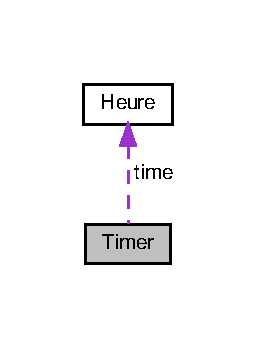
\includegraphics[width=124pt]{structTimer__coll__graph}
\end{center}
\end{figure}
\doxysubsection*{Data Fields}
\begin{DoxyCompactItemize}
\item 
\mbox{\Hypertarget{structTimer_ad6e980d932698bb8fd82498e6c47696c}\label{structTimer_ad6e980d932698bb8fd82498e6c47696c}} 
int {\bfseries start\+Ticks}
\item 
\mbox{\Hypertarget{structTimer_a656a26aa06175d577077ac6181e772fd}\label{structTimer_a656a26aa06175d577077ac6181e772fd}} 
int {\bfseries paused\+Ticks}
\item 
\mbox{\Hypertarget{structTimer_a7fb9c61c8c6b3277fa1a33a054987704}\label{structTimer_a7fb9c61c8c6b3277fa1a33a054987704}} 
int {\bfseries paused}
\item 
\mbox{\Hypertarget{structTimer_ae61fe29f9f0ed5eb7eed278b3dee29f0}\label{structTimer_ae61fe29f9f0ed5eb7eed278b3dee29f0}} 
int {\bfseries started}
\item 
\mbox{\Hypertarget{structTimer_ac7f0cfc2a6dadae0951dd728c60eba69}\label{structTimer_ac7f0cfc2a6dadae0951dd728c60eba69}} 
\mbox{\hyperlink{structHeure}{heure}} {\bfseries time}
\end{DoxyCompactItemize}


The documentation for this struct was generated from the following file\+:\begin{DoxyCompactItemize}
\item 
background.\+h\end{DoxyCompactItemize}

\hypertarget{structVie}{}\doxysection{Vie Struct Reference}
\label{structVie}\index{Vie@{Vie}}
\doxysubsection*{Public Attributes}
\begin{DoxyCompactItemize}
\item 
\mbox{\Hypertarget{structVie_a2656effa8772d33fe9d4d52212db99dc}\label{structVie_a2656effa8772d33fe9d4d52212db99dc}} 
S\+D\+L\+\_\+\+Surface $\ast$ {\bfseries heart}
\item 
\mbox{\Hypertarget{structVie_a7076ab45d1bad6fef6159b35d8056109}\label{structVie_a7076ab45d1bad6fef6159b35d8056109}} 
S\+D\+L\+\_\+\+Rect {\bfseries position\+\_\+heart\+\_\+a}
\item 
\mbox{\Hypertarget{structVie_ac0fc02d542c34723253eeca8cf4b8125}\label{structVie_ac0fc02d542c34723253eeca8cf4b8125}} 
S\+D\+L\+\_\+\+Rect {\bfseries position\+\_\+heart\+\_\+b}
\item 
\mbox{\Hypertarget{structVie_a0398326a6888247e76c1669bf2cd9d11}\label{structVie_a0398326a6888247e76c1669bf2cd9d11}} 
S\+D\+L\+\_\+\+Rect {\bfseries position\+\_\+heart\+\_\+c}
\item 
\mbox{\Hypertarget{structVie_a133255bdd7e91d9c2d90eaf71239540d}\label{structVie_a133255bdd7e91d9c2d90eaf71239540d}} 
int {\bfseries nb\+\_\+vie}
\end{DoxyCompactItemize}


The documentation for this struct was generated from the following file\+:\begin{DoxyCompactItemize}
\item 
hero.\+h\end{DoxyCompactItemize}

%--- End generated contents ---

% Index
\backmatter
\newpage
\phantomsection
\clearemptydoublepage
\addcontentsline{toc}{chapter}{Index}
\printindex

\end{document}
